\clearpage
\appendix
\onecolumngrid
\section*{Supplemental material}
\subsection{Spurious van Hove singularities from gauge non-invariance}
\label{app:supplementalMaterial}

Here we compare our analysis to that of Reference~\cite{Hayashi:2024sae}, which appeared while this work was in preparation. 
First, we note that the target of our analyses differ, in that Reference~\cite{Hayashi:2024sae} 
studied dilepton production in the presence of 
one specific inhomogeneous field configuration: 
a single chiral spiral.  While chiral spirals {\it can}
appear in a moat regime, it is generally not necessary
that they {\it do} appear; indeed, a moat regime need not give
rise to \textit{any} spatially inhomogeneous phase. 
%
Reference \cite{Hayashi:2024sae} 
did not use a gauge invariant form for the higher order derivative terms. Thus their 
$\Gamma^\mu$ does not satisfy the Ward identity of Eq. (\ref{ward_identity}), and the associated photon self energy is not transverse. 
%
Lastly, the new gauge invariant operators to sixth order in the mass dimension, Eqs. (\ref{der_ints1})-(\ref{der_ints4}), are novel to our analysis.

As discussed in the main body of the manuscript, the neglect of higher derivative terms in the vertex leads to the appearance of a van Hove singularity.
To illustrate how the van Hove singularity is smoothed out by
correctly imposing gauge invariance, in Fig.~\ref{fig:gauge} we compute dilepton production in two different ways. 
Both use Eq.~\eqref{eq:dilepton-production} 
at $p=0$, and the dispersion relations in Fig. \ref{fig:dispersionAndDilepton}.
Solid lines represent the correct result, where both the quadratic and quartic terms are gauged; dashed lines are the result where only the quadratic term is gauged. 
For the former, the threshold behavior of pions with a moat is
smooth, like normal pions; for the latter, there are
van Hove singularities, which are thus unphysical at $p=0$.
Neglecting gauge invariance for higher order terms is equivalent to taking $M \rightarrow  \infty$ for the photon-$\phi$-$\phi$ vertex, $\Gamma^\mu$.  
Such a vertex does not satisfy the Ward identity of
Eq.~(\ref{ward_identity}), so the photon
self energy, $\Pi^{\mu \nu}$ is not
transverse, $P^\mu \Pi^{\mu \nu} \neq 0$. 
As described in the main part of the manuscript, the correct vertex structure near threshold, Eq.~\eqref{vertex_canc}, smooths out the van Hove singularity, and leads to the observed enhancement of dilepton production.
%
In Ref. \cite{Hayashi:2024sae}, the integrals over phase space
were modified to eliminate the van Hove singularities.


\begin{figure*}[ht]
    \centering
   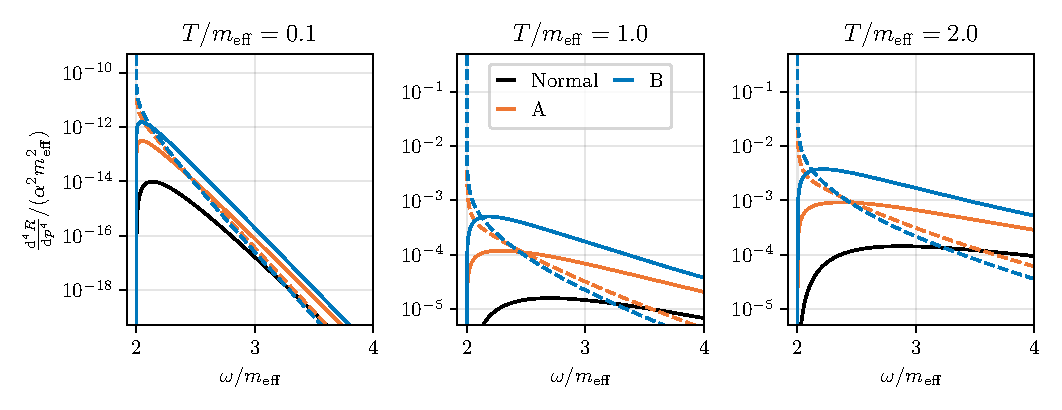
\includegraphics{./dileptonRatePlotTPlots2.pdf}
   \caption{
   Dilepton production rate in Eq.~\eqref{eq:dilepton-production} as a function of $\omega$ at $T/m_\mathrm{eff}=0.1,0.5,1.0$, for the dispersion relations in Fig. \ref{fig:dispersionAndDilepton}, at $\vec p=0$. Solid lines represent the correct result; dashed lines are the result where only the quadratic term is gauged.  }
   \label{fig:gauge}
\end{figure*}

\subsection{Relationship with chiral perturbation theory }

In the main text, we write down a dilepton effective Lagrangian for sigmas and pions, which might prompt one to wonder about the relation between our effective Lagrangian
and other effective theories of light mesons, such as chiral perturbation theory ($\chi$PT) \cite{Gasser:1983yg,Gasser:1984gg}.\\


\noindent{\bf Chiral perturbation theory.} Chiral perturbation theory is a bottom-up effective field theory (EFT) built from light meson fields that respect the global symmetries of QCD and its broken chiral symmetry SU($N_f$)$_L \times$ SU($N_f$)$_R\to $SU($N_f$)$_V$. In the case of $N_f=2$, these are the pions, and in the case of $N_f=3$, we also include kaons and etas.
At lowest order, the $\chi$PT Lagrangian has two terms:
\begin{align}\label{eq:chipt-o2}
{\cal L}_{\chi PT}^{(p^2)}
=\frac{F^2_0}{4}\Tr (\partial_\mu U \partial^\mu U^\dagger)
+\Tr(\chi^\dagger U+U^\dagger\chi)
\end{align}
Here, $U = \exp(i\phi F_0)$ encodes the meson fields in $\phi$ and $\chi$ encodes their masses, which break chiral symmetry.
The pion decay constant $F_0\approx 93$ MeV normalizes the Lagrangian to have the typical kinetic term in $\phi$, as seen from the expansion $U = 1 + i\phi/F_0 + ...\, $.
These fields power count as $U\sim p^0$, $D_\mu U \sim p^1$, $\chi \sim p^2$.

We can write down the most general possible linearly independent set of $\cO(p^4)$ terms of the $\chi$PT Lagrangian as
\begin{align}\label{eq:chipt-o4}
	\cL_{\chi PT}^{(p^4)}& = L_1 \left\{\Tr[D_{\mu}U (D^{\mu}U)^{\dagger}] \right\}^2
%    \nonumber\\
	+ L_2 \,\Tr [D_{\mu}U (D_{\nu}U)^{\dagger}]
	\Tr [D^{\mu}U (D^{\nu}U)^{\dagger}]
 %   \nonumber\\
	+ L_3 \,\Tr[
	D_{\mu}U (D^{\mu}U)^{\dagger}D_{\nu}U (D^{\nu}U)^{\dagger}]
    \nonumber\\
     &+ L_4\, \Tr [ D_{\mu}U (D^{\mu}U)^{\dagger} ]
	\Tr ( \chi U^{\dagger}+ U \chi^{\dagger} )
%   \nonumber\\
	+ L_5 \,\Tr [ D_{\mu}U (D^{\mu}U)^{\dagger}
	(\chi U^{\dagger}+ U \chi^{\dagger})]
 %   \nonumber\\
	+ L_6 [\Tr ( \chi U^{\dagger}+ U \chi^{\dagger}  )
	]^2
    \nonumber\\
    & + L_7\,[ \Tr ( \chi U^{\dagger} - U \chi^{\dagger})]^2
%    \nonumber\\
	 + L_8 \Tr ( U \chi^{\dagger} U \chi^{\dagger}
	+ \chi U^{\dagger} \chi U^{\dagger})
%    \nonumber\\
	 -i L_9 \Tr[ f^R_{\mu\nu} D^{\mu} U (D^{\nu} U)^{\dagger}+ f^L_{\mu\nu} (D^{\mu} U)^{\dagger} D^{\nu} U ]
    \nonumber\\
	& + L_{10}\,\Tr ( U f^L_{\mu\nu} U^{\dagger} f_R^{\mu\nu})\,,
\end{align}
where $L_{1-10}$ are dimensionless constants encoding higher-energy information about QCD that is not described explicitly in $\chi$PT.\\

\noindent \textbf{Bottom-up effective field theory.} 
A rigorous EFT is a description of a system that (1) takes the form of a power expansion, which (2) includes \textit{all} possible relevant operators at a given order that satisfy \textit{all} symmetry conditions imposed on the system \cite{Manohar:2018aog, Iain-EFT, Gross:2022hyw}. An EFT is thus systematically improvable, to an arbitrary degree of precision. There are two types of EFTs: top-down and bottom-up. A top-down EFT is constructed by integrating modes out of $\cL_{\rm QCD}$ systematically, whereas a bottom-up EFT is built from a general operator basis without any assumptions on the nature of the high-energy Lagrangian. We construct a bottom-up EFT from a set of building block fields by writing down the most general set of operators $O_j^{(i)}$ that carry a given power counting (scaling) at each order $\cO(\lambda^i)$. Schematically,
\begin{align}
	&\cL_{\rm EFT} \equiv \cL_{\rm EFT}^{(0)} + \cL_{\rm EFT}^{(1)} + \cL_{\rm EFT}^{(2)} + ...\,,
	&&\cL^{(i)}_{\rm EFT} = \sum_{j} c_j^{(i)}O_j^{(i)}\,.
\end{align}
Here, we determine the couplings $c_j^{(i)}$ by fitting to experiment. 
In EFT, we can generally whittle down the general set of possible $\cO(\lambda^i)$ operators down to a complete, linearly independent set by using the equations of motion \cite{Arzt:1993gz}. It is in general true that \textit{no} new operators must be added at $\cO(\lambda^n)$ when we construct next-order terms of the Lagrangian at $\cO(\lambda^{i+1})$. 
One key difference between a rigorous bottom-up EFT and a bottom-up model is that the EFT considers every single operator possible given these constraints, and is thus uniquely determined, whereas a model includes only some subset of the possible operators.\\


\noindent{\bf Comparison between $\chi$PT and the dilepton effective Lagrangian.}

Let us now compare eq.~\eqref{eq:chipt-o4} to our dilepton Lagrangian in the main text. 
First, it is immediately clear that $\chi$PT and the dilepton Lagrangian are both constructed in the style of a bottom-up effective field theory; however, $\chi$PT is a rigorous EFT of QCD but the dilepton Lagrangian is not. 
An important feature of $\chi$PT is that it is constructed at zero density, and thus describes a Hermitian and Lorentz-invariant system. Thus, we know that we can truncate $\chi$PT at a given order when carrying out precision calculations for collliders and get reasonable results. In contrast, the dilepton Lagrangian is for a non-Hermitian and non-Lorentz-invariant system. When truncating the dilepton expansion at any given order in mass dimension, we have to worry that negative couplings could appear at a higher order than our truncation, and thus that we could miss important effects like additional local minima in the dispersion relation. Writing down the $-Z$ term allows us to  capture the key features of moatons, but is not a systematically improvable choice that could be used in precision studies. Thus we refer to the dilepton Lagrangian as merely an effective Lagrangian and \textit{not} the proper EFT for QCD in a moat regime.
 
Second, we consider the phenomenology. $\chi$PT is an EFT describing the interactions of light mesons at zero density. This contrasts from the models for dilepton production in the main text, which are primarily concerned with a subset of meson fields $\vec{\phi}$ chosen on physical grounds and their effect on the photon field $A_\mu$. Moreover, in the dilepton production case, we are analyzing a dense baryonic system, so we must consider time derivatives and spatial derivatives separately to achieve the full set of linearly independent terms.

Third, let us compare the structure of the two Lagrangians. Although the underlying phenomenology of the two situations is slightly different, we expect that there is a direct relationship between their structure at each order in the power counting. In both cases, we use a set of building block operators that have a parallel power counting structure. Namely, we can draw a comparison $\vec \phi \sim U\sim p^0$, $D_\mu \vec\phi \sim D_\mu U \sim p^1$, and $F_{\mu\nu} \sim f_{\mu\nu}^{L/R}\sim p^2$. On simple algebraic grounds, from two similar sets of building blocks we should construct two similar operator bases for the effective Lagrangian at any given order $\cO(p^{n})$.

Let us see this intuition in action. Comparing the dilepton and $\chi$PT Lagrangians, we immediately notice that we have no equivalent of the $\chi$ field in the dilepton case, and thus we can ignore the terms $L_4$-$L_8$ in eq.~\eqref{eq:chipt-o4}. Next, we recall that the dilepton Lagrangian is at finite density but eq.~\eqref{eq:chipt-o4} describes the behavior of mesons in a vacuum. Thus, a meaningful comparison requires us to take the zero-density limit of the dilepton Lagrangian. In practice, this requires us to set $Z=1$ and combine dilepton terms in which the  time and spatial derivatives are separated. Combining such terms fixes $C_1 = C_2$, $C_3=C_4$, $C_5=C_6$, 
and $C_7=C_8$, 
so that
\begin{align}\label{eq:dilepton-reduce}
    &\cL_{\rm dilepton}^{(p^2,\mu=0)} = \frac{1}{2} (D_\mu \vec{\phi})^2 +  
    \frac{C_1}{M^2} (D_\mu \vec\phi)^2 |\vec\phi|^2
    + \frac{C_3}{M^2} (\vec{\phi}\cdot D_\mu \vec\phi)^2  
    \,,
    \nonumber\\
    &\cL_{\rm dilepton}^{(p^4,\mu=0)} = 
    \frac{1}{2 M^2} (D_\mu^2 \vec{\phi})^2 
 %   \nonumber\\
    + \frac{C_5}{M^2}F_{\mu\nu}^2 |\vec\phi|^2 
  %  \nonumber\\
    + \frac{e C_7}{M^2} F_{\mu\nu} (D_\mu\vec{\phi} \cdot
    i t_2 \cdot D_\nu \vec{\phi})\,.
\end{align}
We immediately see that $C_1$ and $C_3$ align with our $\cO(p^2)$ $\chi$PT Lagrangian. Additionally, two pairs of terms in the $\cO(p^4)$ terms of eqs.~\eqref{eq:dilepton-reduce} and \eqref{eq:chipt-o4} take on similar forms: $(C_5, L_{10})$ and $(C_7, L_9)$.
The terms $L_{1-3}$ contain 4 powers of $D_\mu$, which are reminiscent of the term $(D_\mu^2 \vec{\phi})^2/(2 M^2)$; however, $L_{1-3}$ do not contain an explicit $\Tr[D^2U D^2 U^\dagger]$. Nonetheless, the structure we need can be obtained from these terms by using the equations of motion; specifically, ignoring the $\chi$ terms as previously in $\chi$PT, we have that $  (\partial^2U^\dagger)(\partial^2U)=(\partial_\mu U^\dagger \partial_\mu U)^2$, allowing us to identify $L_1$ with the first term of $\cL_{\rm dilepton}^{(p^4,\mu=0)}$. The terms $L_2$ and $L_3$ do not contribute to the imaginary part of the photon self-energy at lowest order.